% Prezentacja artykułu bazowego (Lab 4, 7.11): 8 slajdów, do 5 minut.
% Kompilacja: latexmk -pdf base_article.tex (obok muszą leżeć wykres_modele.pdf, wykres_warunki.pdf i przyklady.pdf).
% Dane sprawdzone 2.11.2026: strona wydawcy, wykaz ministerialny, Scopus.
\documentclass[aspectratio=169,11pt]{beamer}
\usepackage[T1]{fontenc}
\usepackage[utf8]{inputenc}
\usepackage{polski}
\usepackage{lmodern}
\usepackage{booktabs}
\usepackage{array}
\usepackage{hyperref}

\usetheme{default}
\usecolortheme{seahorse}
\setbeamertemplate{navigation symbols}{}
\setbeamertemplate{footline}[frame number]
\definecolor{akcent}{rgb}{0.2,0.2,0.7}
\setbeamercolor{block title}{bg=akcent!18,fg=akcent!70!black}
\setbeamercolor{block body}{bg=akcent!6}
\setbeamerfont{block title}{size=\small,series=\bfseries}

% Wąska kolumna z etykietą po lewej, bez justowania, bo w wąskich kolumnach rozciąga odstępy.
% Bez \leavevmode kolor przesuwa pierwszy wiersz komórki o linię w dół.
\newcolumntype{L}[1]{>{\raggedright\arraybackslash\leavevmode\color{akcent!70!black}}p{#1}}
\newcolumntype{P}[1]{>{\raggedright\arraybackslash}p{#1}}
\newcommand{\zrodlo}[1]{\par\vfill{\tiny\color{black!65}#1\par}}

\title{Benchmarking OCR and vision-language models for Turkish text recognition: a comprehensive evaluation using synthetic data}
\subtitle{Artykuł bazowy: Y.~Yılmaz, E.~G.~Hanoğlu, A.~G.~Özkan, K.~Öztoprak\\
  \emph{International Journal on Document Analysis and Recognition}, Springer, 2026,
  \href{https://doi.org/10.1007/s10032-026-00613-6}{doi:10.1007/s10032-026-00613-6}}
\author{Marek Siuzdak, Maciej Pietras, Anton Ovod, Paweł Podgórski}
\date{Laboratorium 4, 7.11.2026}

\begin{document}

% 1 --------------------------------------------------------------------------
\begin{frame}
  \titlepage
\end{frame}

% 2 --------------------------------------------------------------------------
\begin{frame}{Czasopismo i autorzy}
  \begin{columns}[T]
    \begin{column}{0.60\textwidth}
      \small
      \begin{tabular}{@{}L{2.15cm}P{5.8cm}@{}}
        Czasopismo & \emph{International Journal on Document Analysis and Recognition} (IJDAR) \\[3pt]
        Wydawnictwo & Springer (Springer Nature) \\[3pt]
        Impact Factor & \textbf{1,7}; pięcioletni 2,3 (2025) \\[3pt]
        Punkty ministerialne & \textbf{100} (wykaz z 5.01.2024, poz. 9473, informatyka techniczna i~telekomunikacja) \\[3pt]
        Tytuł artykułu & \emph{Benchmarking OCR and vision-language models for Turkish text recognition:
          a comprehensive evaluation using synthetic data} \\[3pt]
        Typ artykułu & Original Paper (nowe badania), online od 21.08.2026
      \end{tabular}
    \end{column}
    \begin{column}{0.37\textwidth}
      \small
      \begin{tabular}{@{}lc@{}}
        \toprule
        Autor & Indeks $h$ \\
        \midrule
        Yasin Yılmaz & 0 \\
        Erol Görkem Hanoğlu & 0 \\
        Ayşe Gül Özkan & 5 \\
        Kasım Öztoprak & 9 \\
        \bottomrule
      \end{tabular}

      \vspace{6pt}
      \footnotesize
      Wszyscy: Computer Engineering, Konya Food and Agriculture University, Turcja
    \end{column}
  \end{columns}
  \zrodlo{Źródła: strona czasopisma (Springer), wykaz ministerialny z 5.01.2024, Scopus; stan na 2.11.2026.}
\end{frame}

% 3 --------------------------------------------------------------------------
\begin{frame}{Cel artykułu}
  \begin{itemize}
    \item Modele OCR i~modele wizyjno-językowe (VLM) uczy się głównie na danych z~języków o~dużych zasobach, np.~angielskiego.
    \item Turecki ma mało danych treningowych, siedem liter swoistych (ç, ğ, ı, İ, ö, ş, ü) i~budowę aglutynacyjną, czyli długie słowa.
    \item Wcześniejsze porównania dla tureckiego nie obejmowały VLM, a~brakowało publicznego zbioru z~różnymi zniekształceniami.
  \end{itemize}
  \begin{block}{Cel}
    Pierwsza systematyczna ocena systemów OCR i~modeli VLM w~rozpoznawaniu tekstu tureckiego: wpływ liter tureckich,
    długości słowa, kontekstu zdania, typu tekstu i~zniekształceń oraz przenoszenie wyników z~danych syntetycznych
    na zdjęcia.
  \end{block}
  \medskip
  {\normalsize \textbf{Słowa kluczowe: OCR, VLMs, Turkish text recognition, Synthetic dataset}}
\end{frame}

% 4 --------------------------------------------------------------------------
\begin{frame}{Materiał: zbiór danych}
  \begin{columns}[T]
    \begin{column}{0.47\textwidth}
      \small
      \begin{tabular}{@{}lr@{}}
        \toprule
        Źródło tekstu & Obrazy \\
        \midrule
        \emph{Nutuk} Atatürka, syntetyczne & 6600 \\
        Turecka Wikipedia, syntetyczne & 6600 \\
        \emph{Gold Standard}, zdjęcia & 90 \\
        \bottomrule
      \end{tabular}

      \smallskip
      Druk (13 krojów, tła papieru), pismo odręczne (340 fontów Google Fonts), tekst w~scenie (tła COCO).
      Generator TRDG~1.8.0 i~własne skrypty. Zdjęcia: 6~podkategorii po~15, bez zniekształceń.
    \end{column}
    \begin{column}{0.50\textwidth}
      \small
      \begin{tabular}{@{}L{2.4cm}P{4.1cm}@{}}
        \toprule
        Kategoria & Podkategorie \\
        \midrule
        Litery tureckie & z~nimi, bez nich \\[1pt]
        Długość słowa & poniżej 10, ponad 10 znaków \\[1pt]
        Kontekst & pojedyncze słowo, zdanie \\[1pt]
        Zniekształcenia & czysty, obrót, szum, rozmycie, niska rozdzielczość (te same teksty) \\
        \bottomrule
      \end{tabular}

      \smallskip
      {\footnotesize 3 typy $\times$ 11 podkategorii $\times$ 200 obrazów = \textbf{6600}\par}
    \end{column}
  \end{columns}

  \vspace{4pt}
  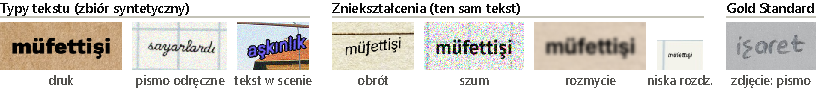
\includegraphics[width=\textwidth]{przyklady.pdf}
  \zrodlo{Przykłady: zbiór autorów na Zenodo, DOI 10.5281/zenodo.21923181 (CC~BY~4.0), część Wikipedia i~Gold Standard.}
\end{frame}

% 5 --------------------------------------------------------------------------
\begin{frame}{Metody: modele i ocena}
  \begin{columns}[T]
    \begin{column}{0.45\textwidth}
      \small
      10 modeli bez douczania na tureckim:

      \smallskip
      \begin{tabular}{@{}L{1.75cm}P{4.1cm}@{}}
        \toprule
        OCR & PaddleOCR, TrOCR, GOT-OCR 2.0 \\[2pt]
        Otwarte VLM & Qwen2.5-VL 7B, InternVL3 8B, DeepSeek-VL2 Tiny, Phi-3.5-Vision, Pixtral 12B \\[2pt]
        Komercyjne VLM & GPT-4o, Claude Sonnet 4 (przez API) \\
        \bottomrule
      \end{tabular}

      \medskip
      Google Colab, GPU Nvidia A100; każdy model odczytuje 13\,200 + 90 obrazów.
    \end{column}
    \begin{column}{0.52\textwidth}
      \small
      \begin{itemize}
        \item Polecenie dla VLM: \emph{,,Extract the Turkish text from the image exactly as it appears\ldots''};
          odpowiedzi z~komentarzem powtórzono z~ostrzejszym poleceniem (74 przypadki, 0,56\%).
        \item Miary: CER $=(S+D+I)/N$ (główna) i~WER (tylko zdania).
        \item Przed liczeniem małe litery (TrOCR zwraca same wielkie), CER obcięty do 1.
        \item Statystyka: bootstrap 95\% (1000 losowań), korelacja Spearmana między zdjęciami a~danymi syntetycznymi.
        \item Litery tureckie: dopasowanie Levenshteina.
      \end{itemize}
    \end{column}
  \end{columns}
\end{frame}

% 6 --------------------------------------------------------------------------
\begin{frame}{Wyniki: porównanie modeli}
  \begin{columns}[T]
    \begin{column}{0.62\textwidth}
      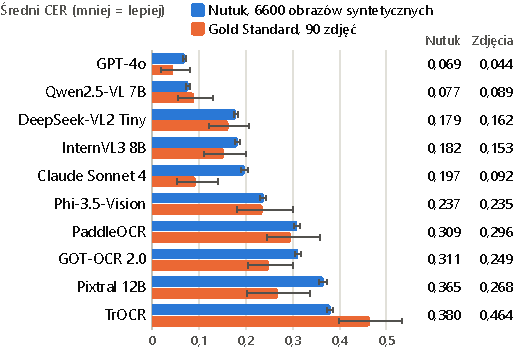
\includegraphics[width=\textwidth]{wykres_modele.pdf}
    \end{column}
    \begin{column}{0.36\textwidth}
      \small
      \begin{itemize}
        \item GPT-4o i~otwarty Qwen2.5-VL wyraźnie przed resztą.
        \item Claude Sonnet 4 dopiero piąty (0,197), na zdjęciach trzeci (0,092).
        \item TrOCR ostatni na obu zbiorach.
        \item Kolejność na zdjęciach zgodna z~syntetyczną: $\rho=0{,}92$, $p<0{,}001$.
        \item Wikipedia: CER średnio o~3\% wyższy, kolejność prawie bez zmian.
      \end{itemize}
    \end{column}
  \end{columns}
  \zrodlo{Wartości odczytane z~rys. 3 i~11 artykułu; kreski: przedziały 95\% (bootstrap).}
\end{frame}

% 7 --------------------------------------------------------------------------
\begin{frame}{Wyniki: co utrudnia odczyt (zbiór Nutuk)}
  % Klamra zaraz po tytule ramki zostałaby podtytułem, dlatego \centerline.
  \centerline{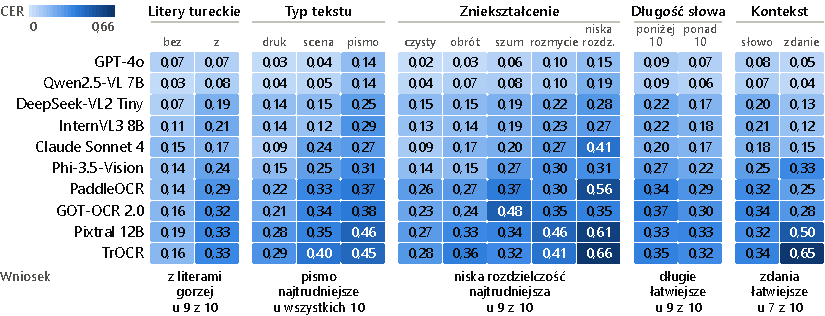
\includegraphics[width=0.95\textwidth]{wykres_warunki.pdf}}
  \small
  \begin{itemize}
    \item Litery tureckie odczytane poprawnie: GPT-4o 86-94\%, Qwen2.5-VL 73-93\%, Claude Sonnet 4 69-78\%,
      GOT-OCR 3-5\%, TrOCR i~PaddleOCR prawie 0\%; najtrudniejsze ı~i~İ.
    \item WER zdań: GPT-4o 0,11 i~Qwen2.5-VL 0,12 wobec 0,83 (GOT-OCR) i~0,87 (TrOCR).
  \end{itemize}
  \zrodlo{Wartości odczytane z~rys. 4-9 i~14 artykułu.}
\end{frame}

% 8 --------------------------------------------------------------------------
\begin{frame}{Wkład autorów, nowości i~nasza replikacja}
  \begin{columns}[T]
    \begin{column}{0.48\textwidth}
      \begin{block}{Artykuł bazowy: wkład i nowości}
        \small
        \setlength{\leftmargini}{1.2em}
        \begin{itemize}
          \setlength{\itemsep}{0pt}
          \item Pierwszy benchmark OCR i~VLM dla tureckiego (zniekształcenia, kontekst).
          \item Publiczny zbiór 13\,200 obrazów (druk, pismo, scena) oraz 90 zdjęć.
          \item Analiza 7 liter tureckich i~ocena 10 modeli.
          \item Walidacja na zdjęciach: $\rho=0{,}92$ ($p<0{,}001$).
        \end{itemize}
      \end{block}
      \vspace{2pt}
      {\scriptsize \textbf{Ograniczenia wg autorów:} pismo z~fontów zamiast odręcznego, brak dostrajania, mały zbiór zdjęć (90 szt.).\par}
    \end{column}
    \begin{column}{0.48\textwidth}
      \begin{block}{Nasz wkład: replikacja na Colabie}
        \small
        \setlength{\leftmargini}{1.2em}
        \begin{itemize}
          \setlength{\itemsep}{0pt}
          \item Weryfikacja 65\,036 wartości CER z~plików autorów (pełna zgodność).
          \item \textbf{Uruchomienie 8 modeli na GPU A100} (próbka 1650 obrazów, po 50 na komórkę).
          \item \textbf{Średni CER zgodny do 0,001} (Pixtral 0,007 z~braku stałego ziarna).
          \item Identyczność predykcji: 90,4--100\%.
        \end{itemize}
      \end{block}
    \end{column}
  \end{columns}
  \zrodlo{Dane autorów: Zenodo (CC~BY~4.0), kod: GitHub. Nasze kody i wyniki replikacji: w dołączonym repozytorium.}
\end{frame}

\end{document}
